\documentclass{article}
\usepackage[a4paper, top=2.5cm, bottom=2.5cm, left=2.5cm, right=2.5cm]{geometry}

\usepackage[utf8]{inputenc}

\usepackage{graphicx}
\usepackage{caption}
\usepackage{subcaption}
\usepackage{float}
\usepackage{amsmath}

\usepackage{pgfplots}
\pgfplotsset{compat=1.18}

\usepackage{minted}
\usepackage{hyperref}

\begin{document}

\title{
  \textbf{SDC Assignment 2 - ITRI Dataset Visualization}
}
\author{Ying Pei Lin}
\date{Spring 2026}

\maketitle

\section*{Task 1: Rosbag Information}

\begin{figure}[H]
    \centering
    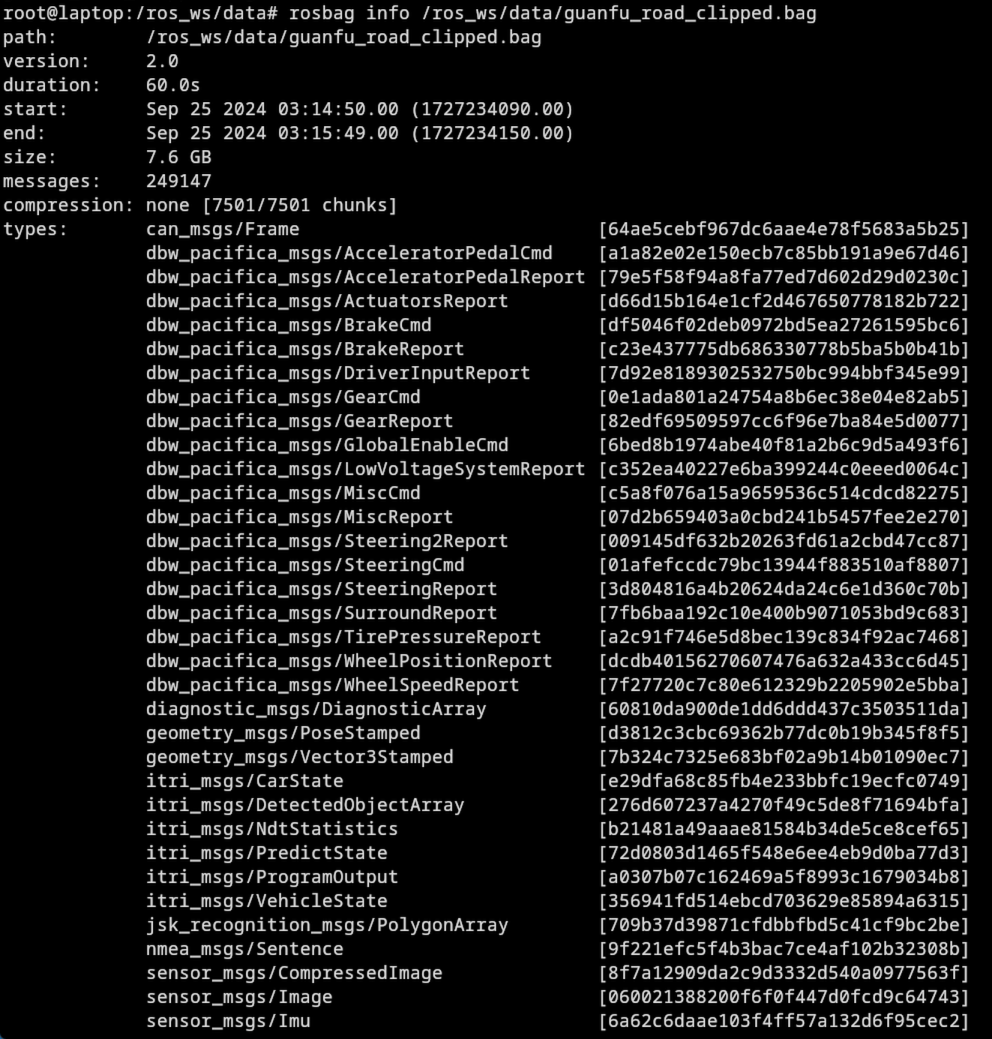
\includegraphics[width=1.0\textwidth]{t1-baginfo-1.png}
    \caption{Bag Info Part 1}
\end{figure}

\begin{figure}[H]
    \centering
    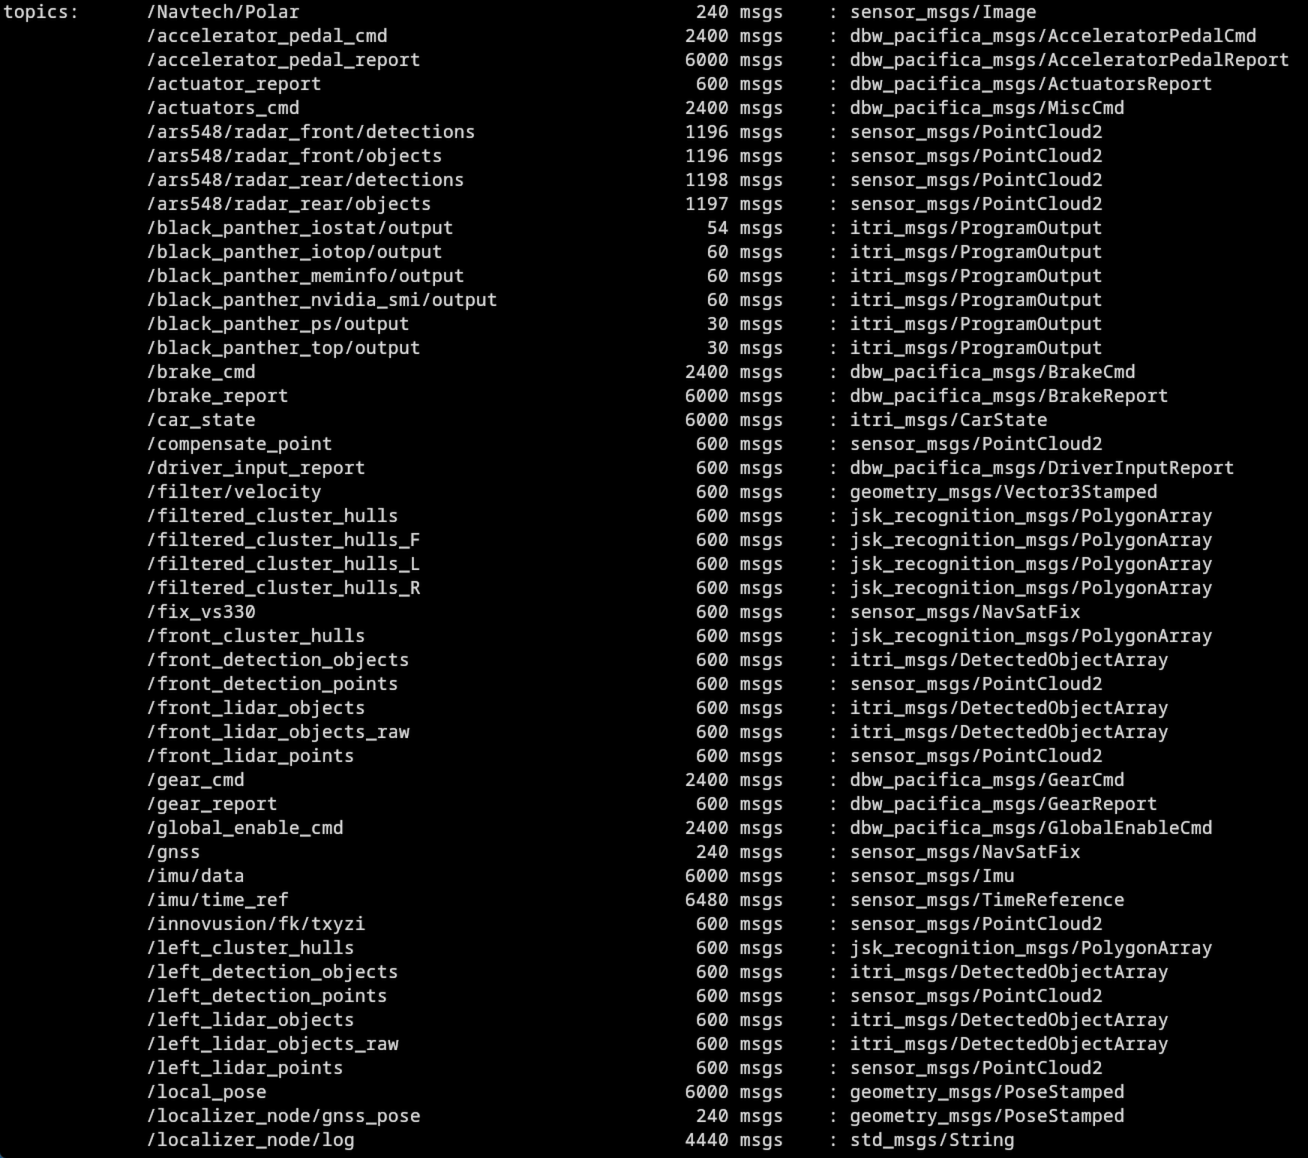
\includegraphics[width=1.0\textwidth]{t1-baginfo-2.png}
    \caption{Bag Info Part 2}
\end{figure}

\begin{figure}[H]
    \centering
    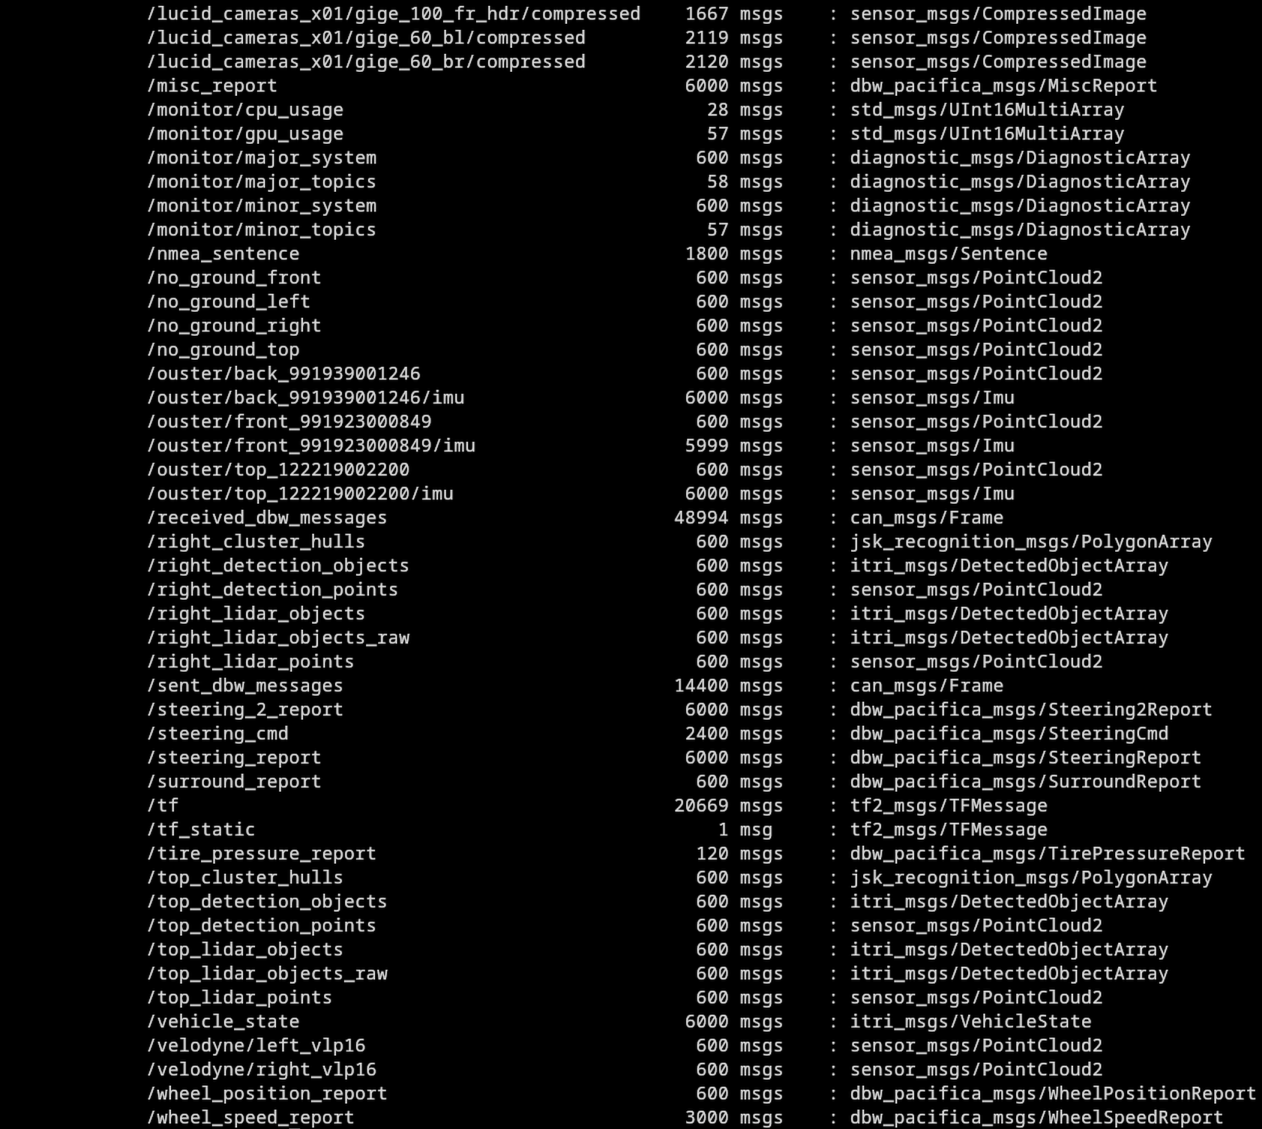
\includegraphics[width=1.0\textwidth]{t1-baginfo-3.png}
    \caption{Bag Info Part 3}
\end{figure}

\section*{Task2: Point Cloud Topic Information}

\begin{figure}[H]
    \centering
    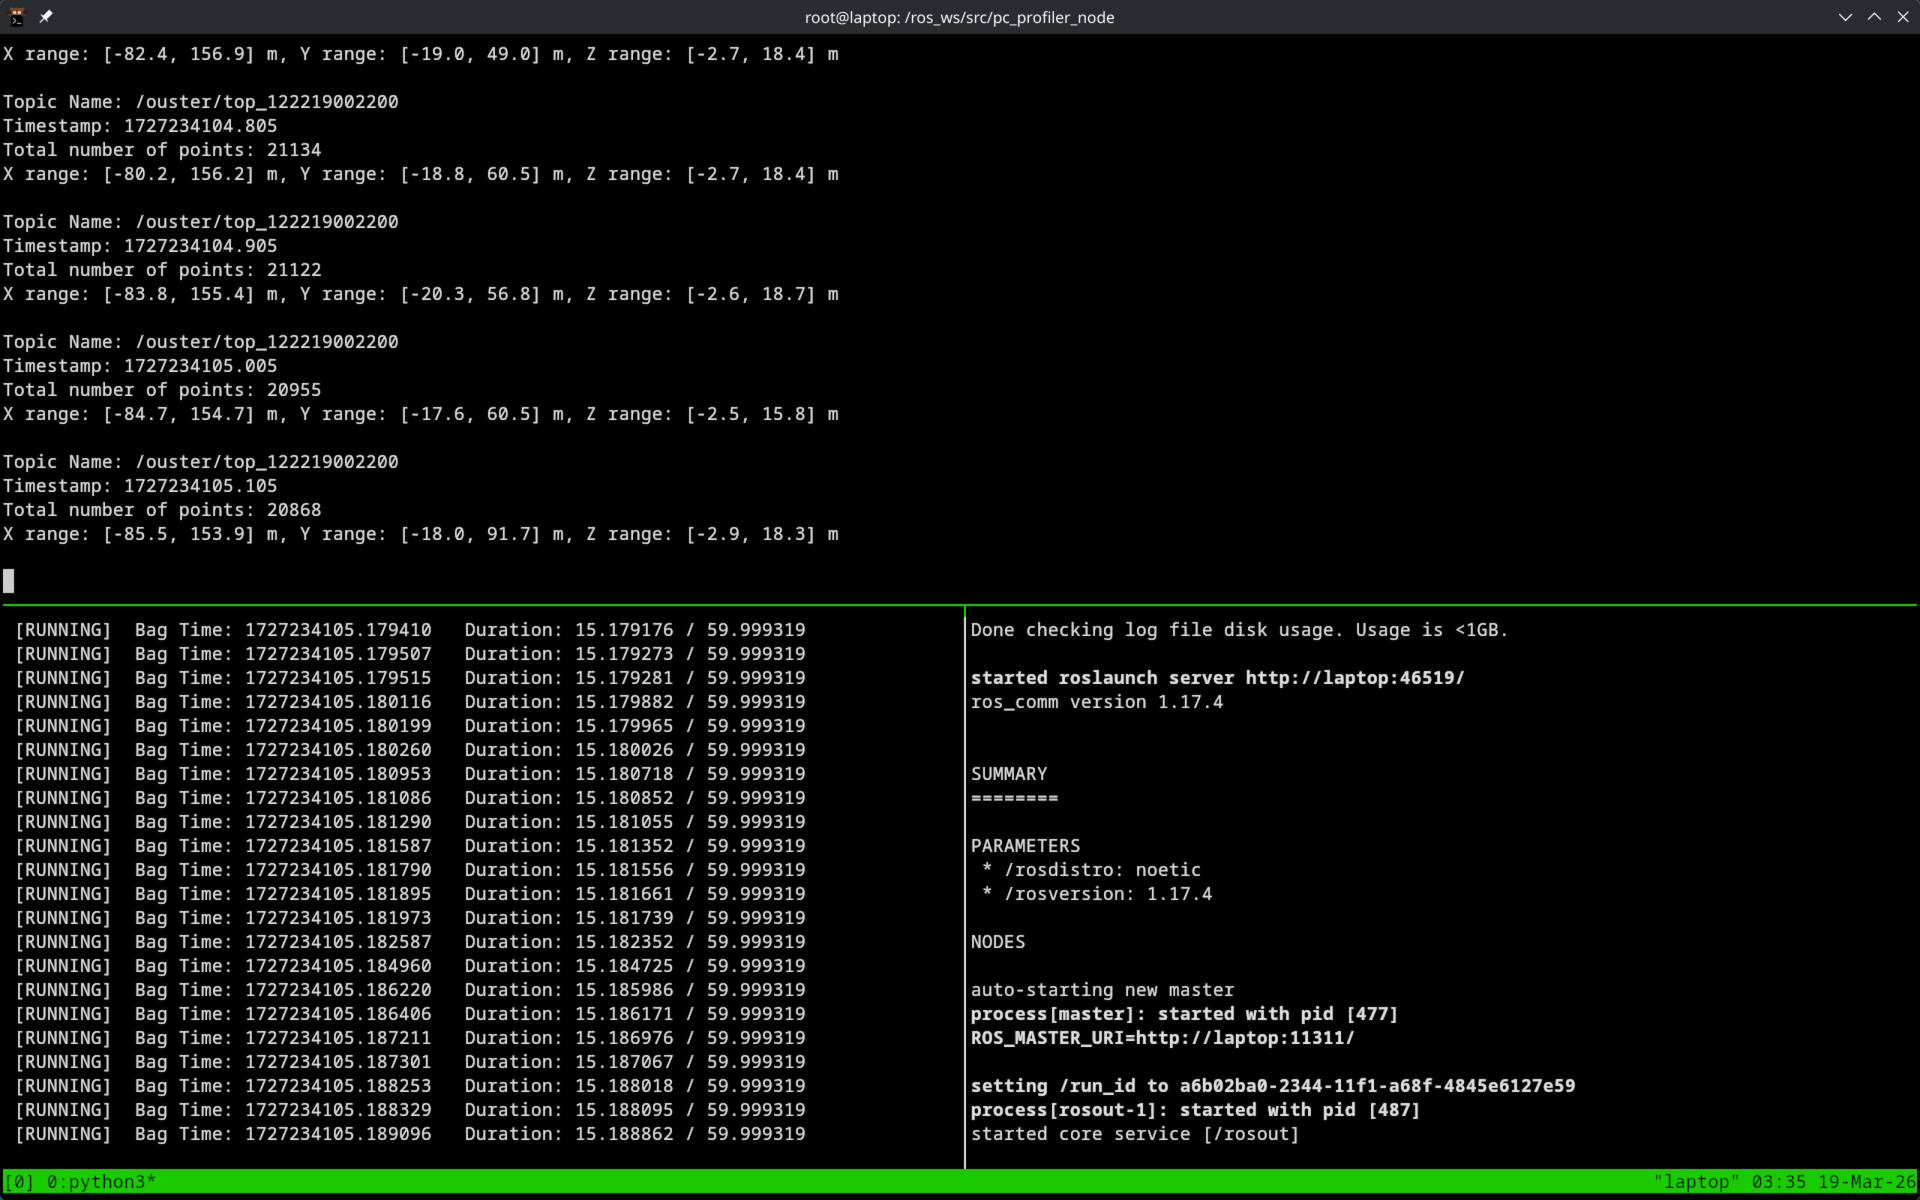
\includegraphics[width=1.0\textwidth]{t2-lidar.png}
    \caption{Terminal output of pc\_profiler.py for LiDAR (/ouster/top\_122219002200)}
\end{figure}

\begin{figure}[H]
    \centering
    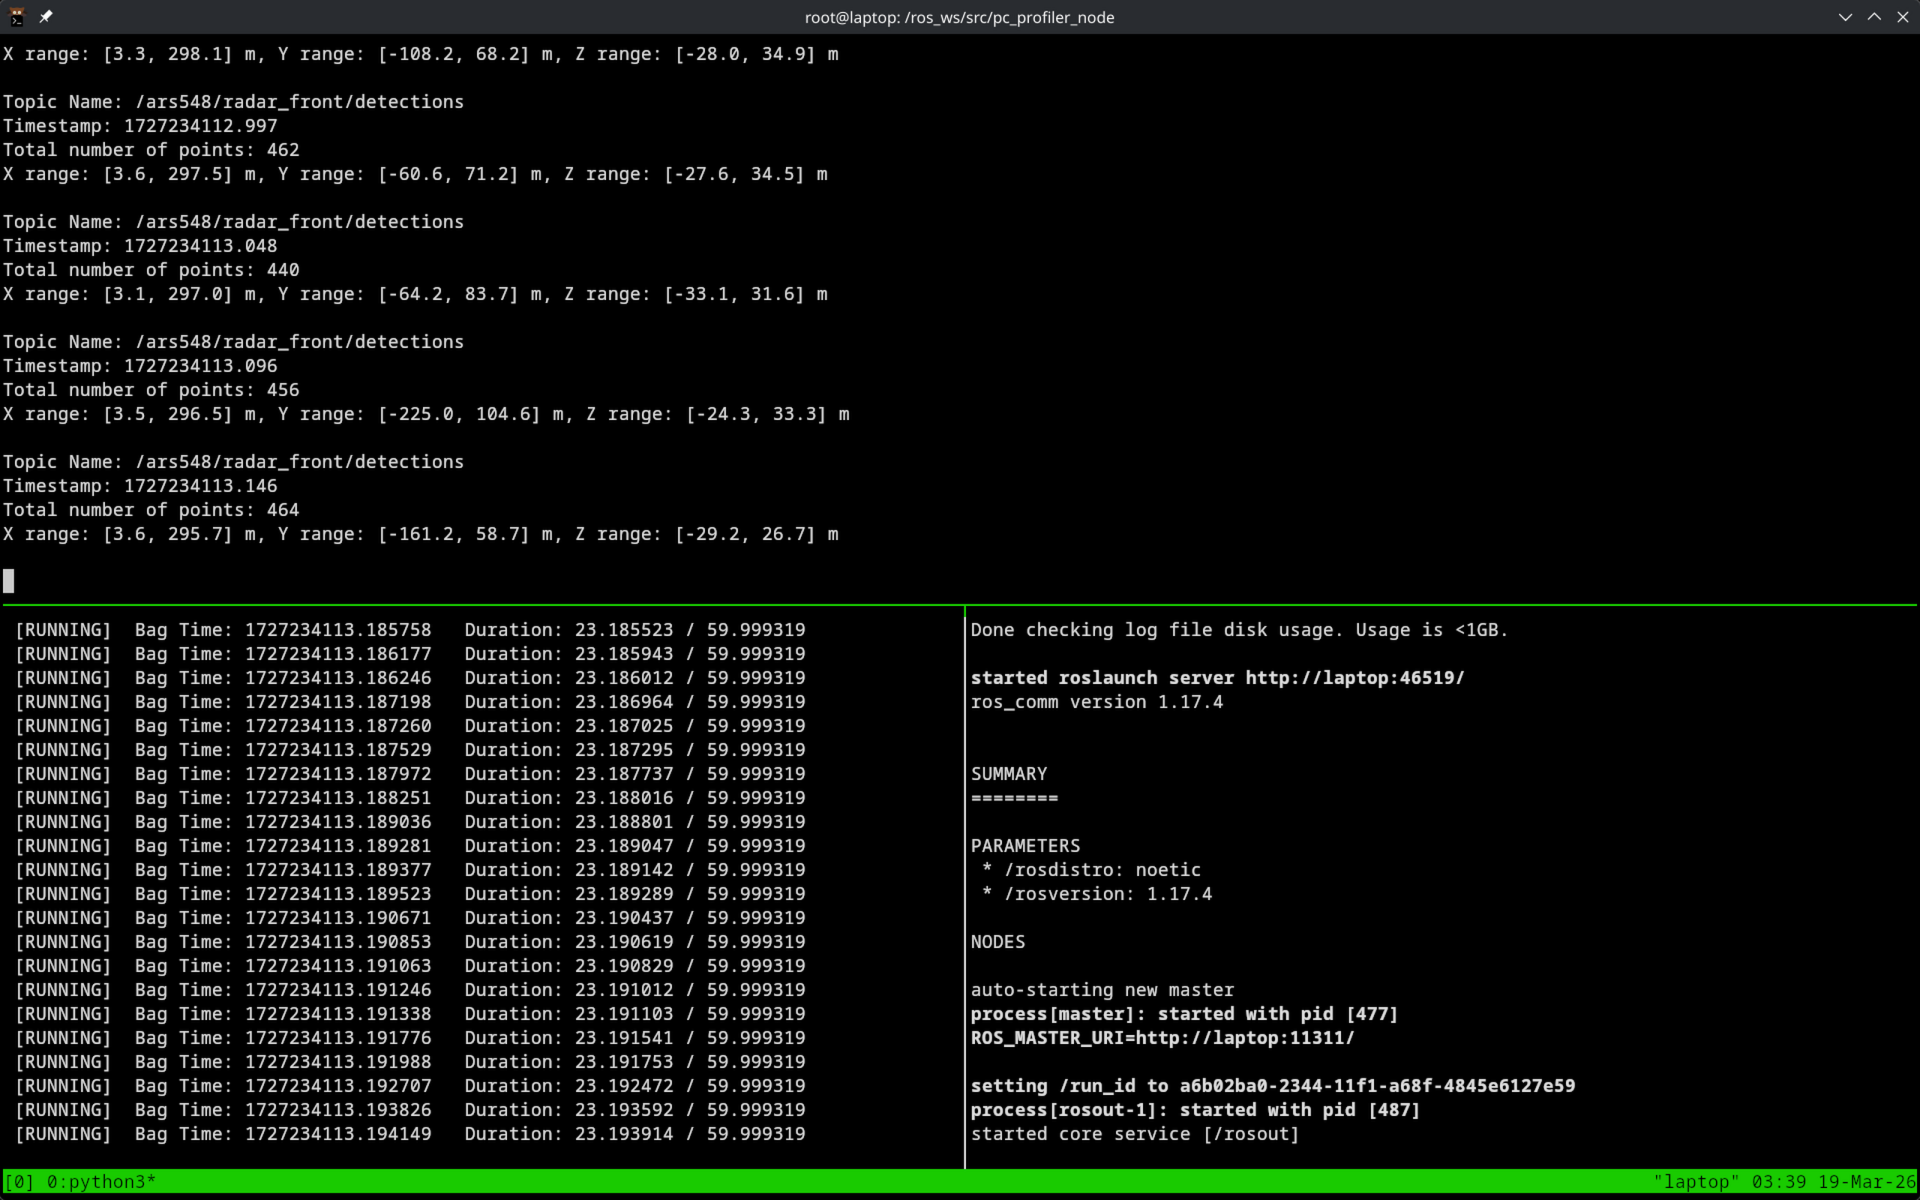
\includegraphics[width=1.0\textwidth]{t2-radar.png}
    \caption{Terminal output of pc\_profiler.py for Radar (/ars548/radar\_front/detections)}
\end{figure}

\section*{Task 3: Visualization of Rosbag Data}

\begin{figure}[H]
    \centering
    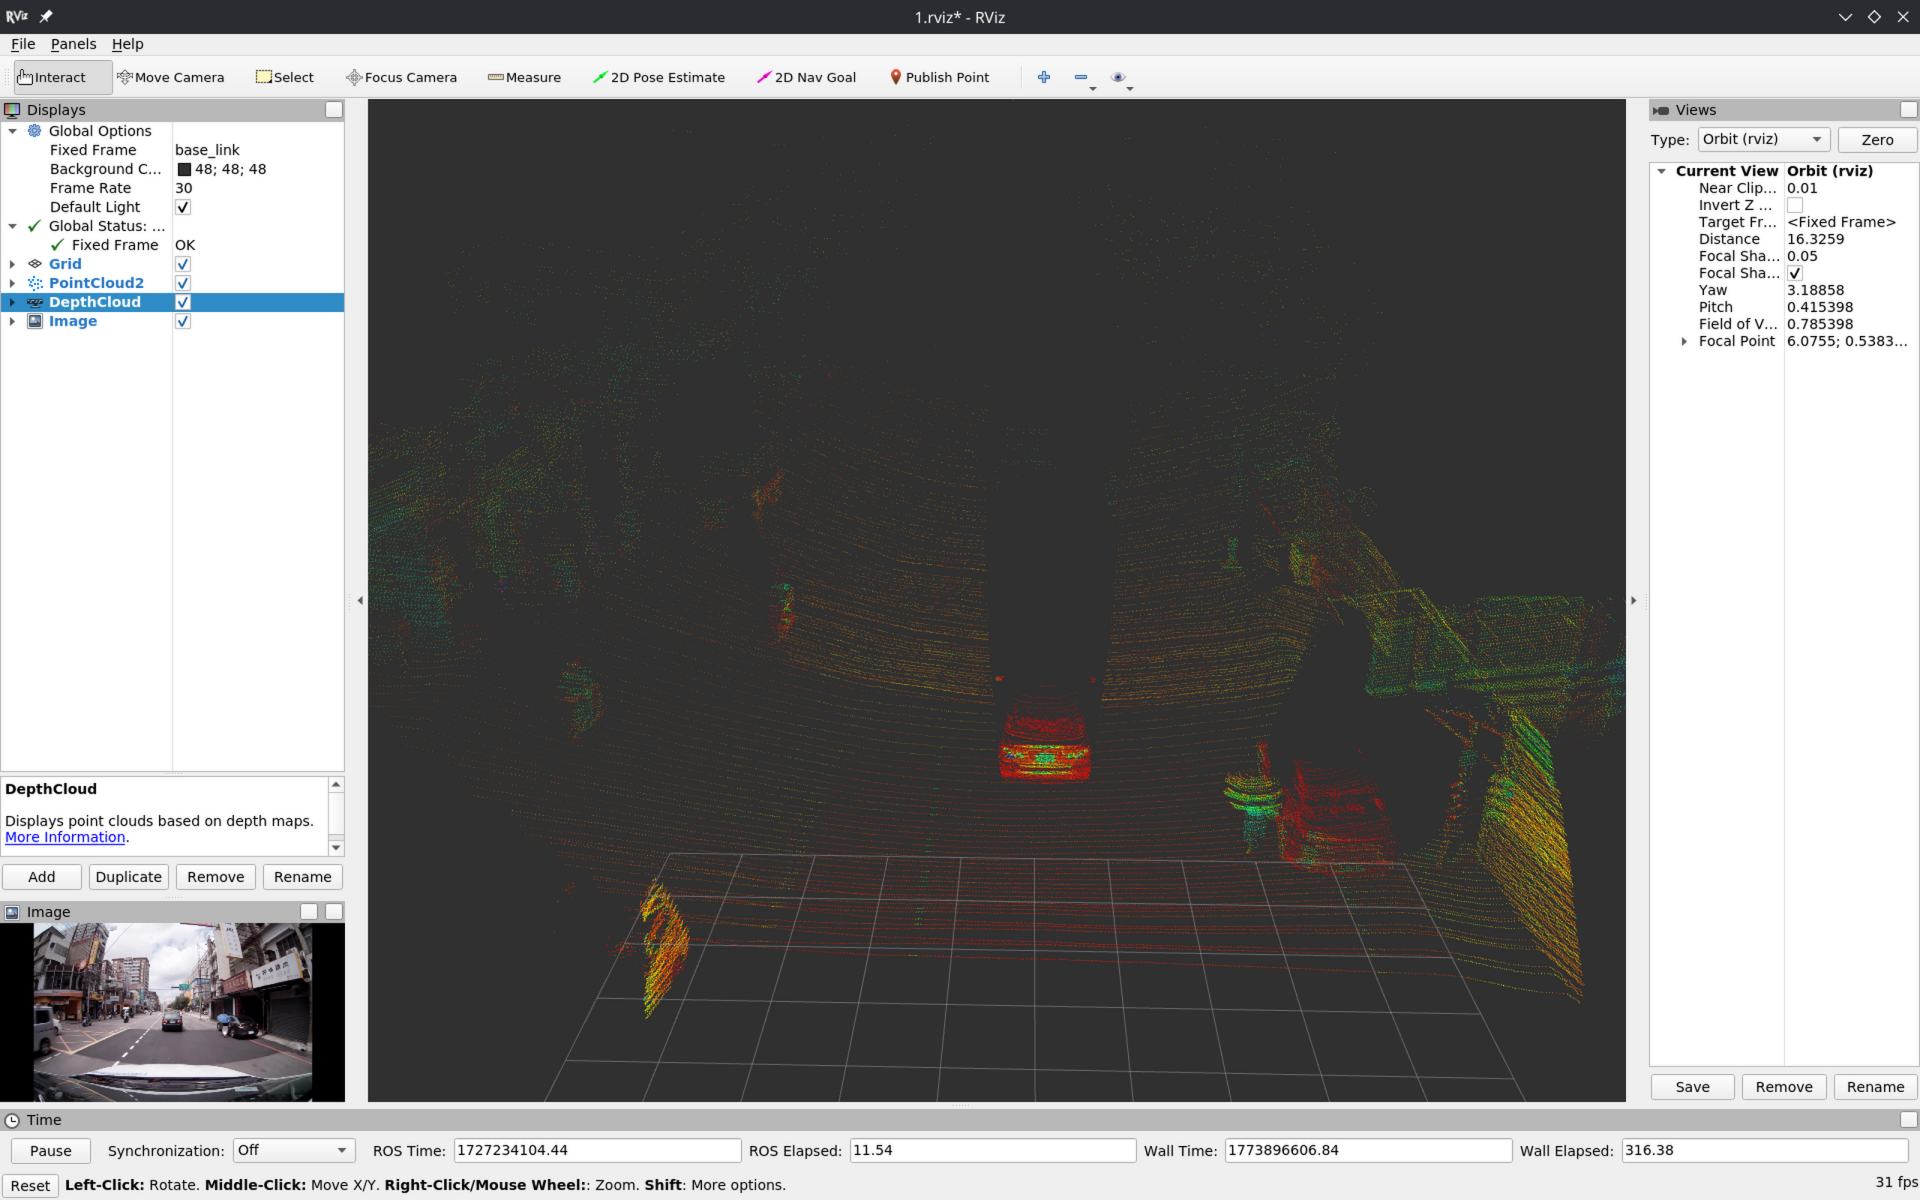
\includegraphics[width=1.0\textwidth]{t3.png}
    \caption{RViz pointcloud showcasing high-reflectivity objects alongside the camera image.}
\end{figure}

\section*{Task 4: Radar Relative Speed Visualization}

\textbf{YouTube Link:} \url{https://youtu.be/jN5-tlbwZaI?si=e-uYSNdmzpDiPUll}

\section*{Task 5: How does LiDAR measure distance?}

LiDAR (Light Detection and Ranging) measures distance using the \textbf{Time of Flight (ToF)} principle. The sensor emits a short laser pulse and simultaneously starts a timer. When the light reflects off an object and returns to a photodetector, the timer stops. The distance ($d$) is calculated using the constant speed of light ($c \approx 3 \times 10^8$ m/s) and the exact time interval ($\Delta t$) of the round trip:
$$ d = \frac{c \cdot \Delta t}{2} $$

To achieve the centimeter-level accuracy needed for autonomous driving, this time interval must be measured with picosecond ($10^{-12}$ s) precision. This is accomplished using a specialized integrated circuit called a \textbf{Time-to-Digital Converter (TDC)}. The laser firing triggers a high-speed "START" electrical signal, and the returning photons hitting the photodetector generate a "STOP" signal. The TDC acts as an ultra-fast hardware stopwatch, precisely measuring the microscopic gap between these two pulses and translating it into a digital distance value.
\end{document}
